\section{Generation of Calibrated Radiances}
\label{sec:5.2:CalibratedRadiances}

ALI arrived back in Saskatoon on September 25, of 2015 and was unpacked and checked for any damages from either the transportation back to Saskatoon or from the landing at the end of the mission. No obvious damage had occurred to ALI and the instrument was functioning correctly. This allowed the complete data set record by ALI to be downloaded and used for aerosol profile processing. This section will undergo the method used to convert the raw data from the CCD to measured relative radiances used in the retrieval process.

The raw flight data, known as the level 0 data, must be converted to into level 1 relative radiances, which is the data normalized to a laboratory measurement value, before they can be used to retrieve aerosol extinction and particle size. The transformation includes removal of dark current, DC bias, stray light, and application of flat fielding calibration.

The DC offset is an bias that is applied to the analogue digital converter inside the CCD camera that causes a bias in the final count values for the image. This need to be removed in order to be able to get the pure measurement counts from the instrument. It is usually assumed that the DC offset for a CCD is a constant across the operating temperatures and exposure times of the device, however the DC offset for the camera used in ALI exhibited a temperature dependance. By using the dark images from the assent of the flight which was in darkness combined with laboratory dark images all of which were takeing at the shortest possible exposure time of the camera to remove contribution from dark current. From using this set a data a curve was determined to fit the DC offset with respect to temperature and the curve is in the form of
\begin{equation}
    \text{DC offset} = 0.00659T^{3}-0.09202T^{2}-3.5368T+643.5127
    \label{eqn:5.2:DcOffsetCurve}
\end{equation}
where $T$ is the CCD temperature as measure from the CCD temperature sensor in degrees Celsius and is plotted in \autoref{fig:5.2:dcOffsetCurve}. The dark current is the thermal energy that builds up in the CCD pixels that grows linearly with exposure time and temperature. For the operating temperatures of ALI combined with the short exposure times used during the mission lead to the system having a very small dark current contribution in the measurement images. The dark current was as small as a single count to at most seven counts for the worst case scenario (longest exposure time and hottest temperature.) Since this correct was small compared to the DC offset and the final counts the dark current was added as a a noise contribution for the images. At this point all the non-exposure time sensitive components had been removed and all the images were converted from counts to counts per second by divided the corrected counts by the exposure time.
 %by taking the counts in the image and divided by the exposure time, in order to easily relate the radiance of different images directly to each other without having to scale the results with respect to the exposure time.

\begin{figure}
    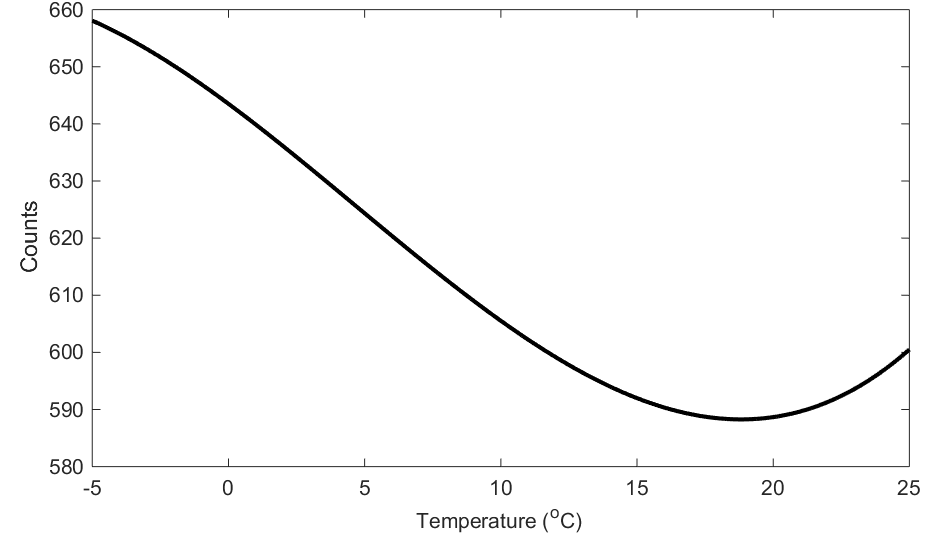
\includegraphics[width=1.0\textwidth]{./Images/5-2-DcOffset.pdf}
    \caption[Determined ALI DC Offset]{The determined DC offset determined for ALI in the form seen in \autoref{eqn:5.2:DcOffsetCurve}. The counts on the vertical axis os the counted that need to be removed to remove the DC offset.}
    \label{fig:5.2:dcOffsetCurve}
\end{figure}

Stray light removal has always been difficult in atmospheric instrumentation due to the difficulty in accurately discerning the signal in regards to the stray light contamination. Furthermore, ALI's optical system has the further addition of unwanted light internal to the instrument because of the rejection of one of the polarizations due to the nature of the AOTF. The signal enters the optical system unpolarized, but only one polarization can have a consistent output angle from the AOTF. The entering light is passed through a linear polarizer with an extinction ratio of at least 100,000:1 to remove the unwanted polarization however a small percentage is not absorbed. Furthermore, a second linear polarizer is used after the AOTF to reject all of the unwanted radiance that did not meet the Bragg criteria and once again a small percentage of this radiance is not absorbed. Since only a very small wavelength bandpass composses the wanted signal even small component of the unwanted signal passing through the system adds a considerable amount of stray light. However, the active filtering of the AOTF allows for an image to be measured when the filtering device is disabled, which is with no applied RF, allowing only the stray light to be captured by the instrument which will be referred to as a `dark image'. During ALI's aerosol mode a `dark image' was captured before every measurement image. By removing the `dark images' from the signal-stray light contaminated images the end result is images that only contain the measured signal. The previous method was tested in the lab with a known source with even illumination across the field of view of the system, the resulting final image is left with a even decrease in intensity radiating from the center of the field of view as its expected with the known vignetting of ALI. The vignetting is caused by the aperture of the AOTF itself, by using a simple optical layout as chosen for the prototype the larger the angle for the field of view the more light that get blocked by the AOTF's aperture causing a known vignetting for the images. Furthermore the exterme range of the field of view, approximately the last one degree, is outside the acceptance angle of the AOTF which causes a loss of diffraction efficiency. Both of these effect will also need to be calibrated out of the measurements.

ADD FIGURE ABOUT STRAY LIGHT

To finalize the data into level 1 relative radiances a flat fielding calibration is preformed, which involves taking all the incoming fielding of views and normalize them to be unity. The flat fielding coefficients needed to be applied not only spatially across each image but spectrally across a series of images. To determine the flat fielding coefficients ALI was set up in the lab viewing the light emitted from a 250~W quartz-tungsten halogen bulb that is passed through a diffusing plate to give an evenly distributed signal across the entire field of view of ALI. Measurements were taken at varying integration times at every wavelengths used in ALI's aerosol mode. Since ALI is most sensitive at 750~nm, it was chosen to be the reference point. The center pixels of the 750~nm images were used since they experience little vignetting, specifically the center 25 by 25 pixels. All pixels for every image were normalized to the mean of the reference point pixels. From these normalized images, the flat fielding coefficients were the values needed to multiply the normalized images to achieve unity. The coefficients were then averaged for each wavelength and applied to the flight data to yield the final relative radiances. In \autoref{fig:5.2:BeforeAfterImages} image number 212, a 750~nm image, is shown with a before and after comparison. The before image is the raw data directly after the mission with no calibrations preformed and the after image in the bottom panel is the same image after the all the calibrations have been applied.

\begin{figure}
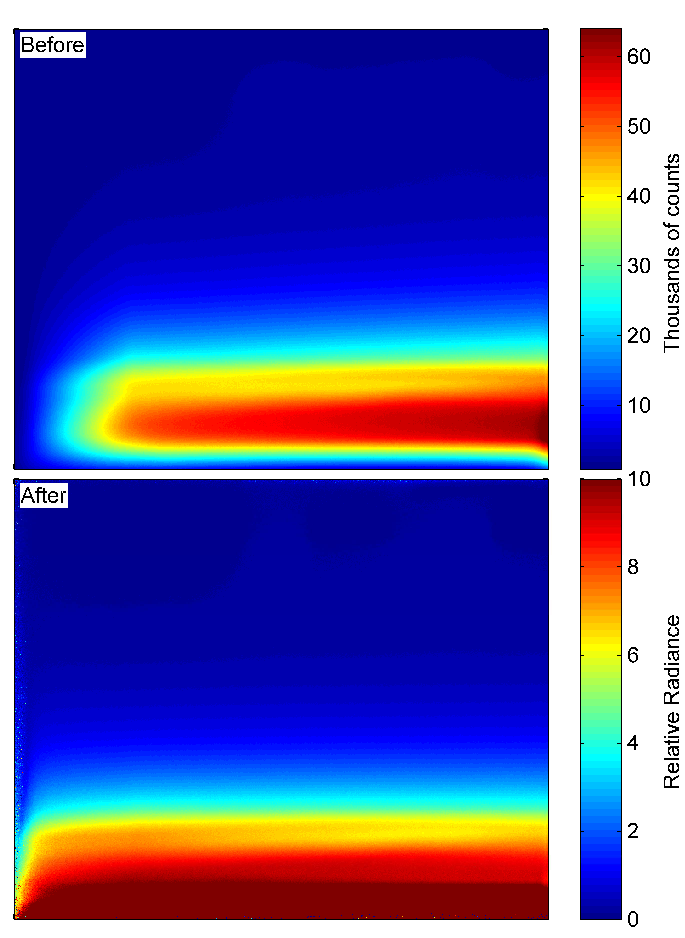
\includegraphics[width=1.0\textwidth]{./Images/5-2-BeforeAfterImage.pdf}
    \caption[Comparison of an Raw and Calibrated ALI Image]{Comparison of the same image, image number 212, at 750~nm. The upper panel is the raw level 0 data and the lower panel is the relative radiance level 1 data.}
    \label{fig:5.2:BeforeAfterImages}
\end{figure}

%and used to normalized the full field of view across the whole spectrum to the center of the 750~nm images, thus giving a relative calibration of radiance referenced to this point. The process used to determine the flat fielding coefficients started with similar process used to remove the stray light during the mission post processing. The images had the DC bias and dark current removed for proper unbiased comparisons and converted to counts per second. Each value of every pixel in the active region of the CCD was normalized to the mean of the value on the center 25 by 25 pixels at 750~nm over all exposure times and trials. The coefficients for flat fielding can be determined as the values to yield a unified radiances of one across all field of views and wavelengths. These coefficients are then applied to the data from the flight that give relative radiances for each pixel.

To increase the precision of the measurements from the flight the images were averaged in cells of 25 horizontal pixels and vertical pixel averaging that would result in the measured radiances being on a 1~km vertical grid. Furthermore, a loss of resolution was speculated to occur in the flight data because of the drastic change in temperature of the optics during the flight which is a secondary reason for the pixel averaging. ALI radiance profiles from the complete mission from the 0\si{\degree} line of sight can be seen in \autoref{fig:AliRadiancesVectors} which includes wavelengths from 675-950~nm and generally have good internal agreement from 13 to 30~km. Images 207, 211, and 215 were selected to demonstrate subtle radiance differences between different horizontal lines of sights with each profile's respective error and can be seen in \autoref{fig:AliRadiances}. Lastly, images 204 to 216 were used to show the spectrum of relative radiances at a series of altitudes which is seen in \autoref{fig:AliSpectralRadiances}.

\begin{figure}
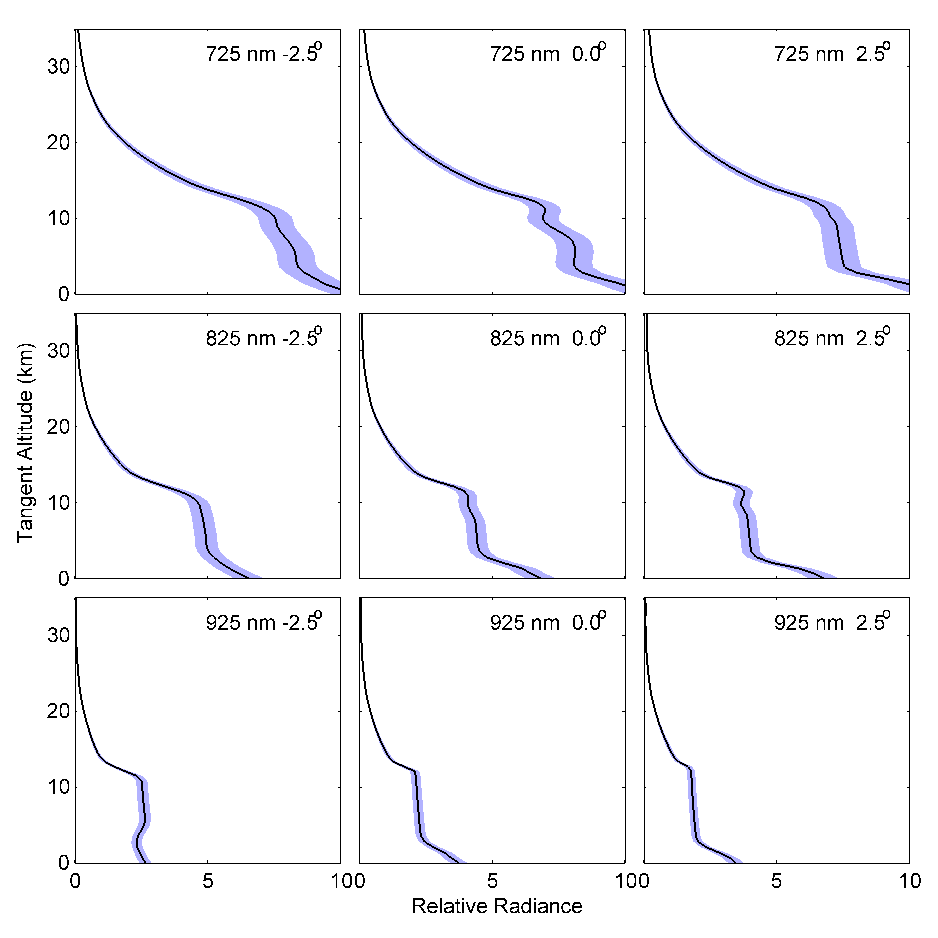
\includegraphics[width=1.0\textwidth]{./Images/5-2-AliRadiances.pdf}
    \caption[TODO:Write This]{Level 1 relative radiances as measured form ALI at approximately 14:20 UTC (images number 207, 211,and 215) looking 90\si{\degree} from the sun facing southwards. The top middle, and bottom row are measurements taken at 725, 825, and 925~nm respectively. The center column is viewing the atmosphere directly in front of ALI, While the left column is looking to the left at -2.5\si{\degree} and the right at 2.5\si{\degree}. }
    \label{fig:5.2:AliRadiances}
\end{figure}

\begin{figure}
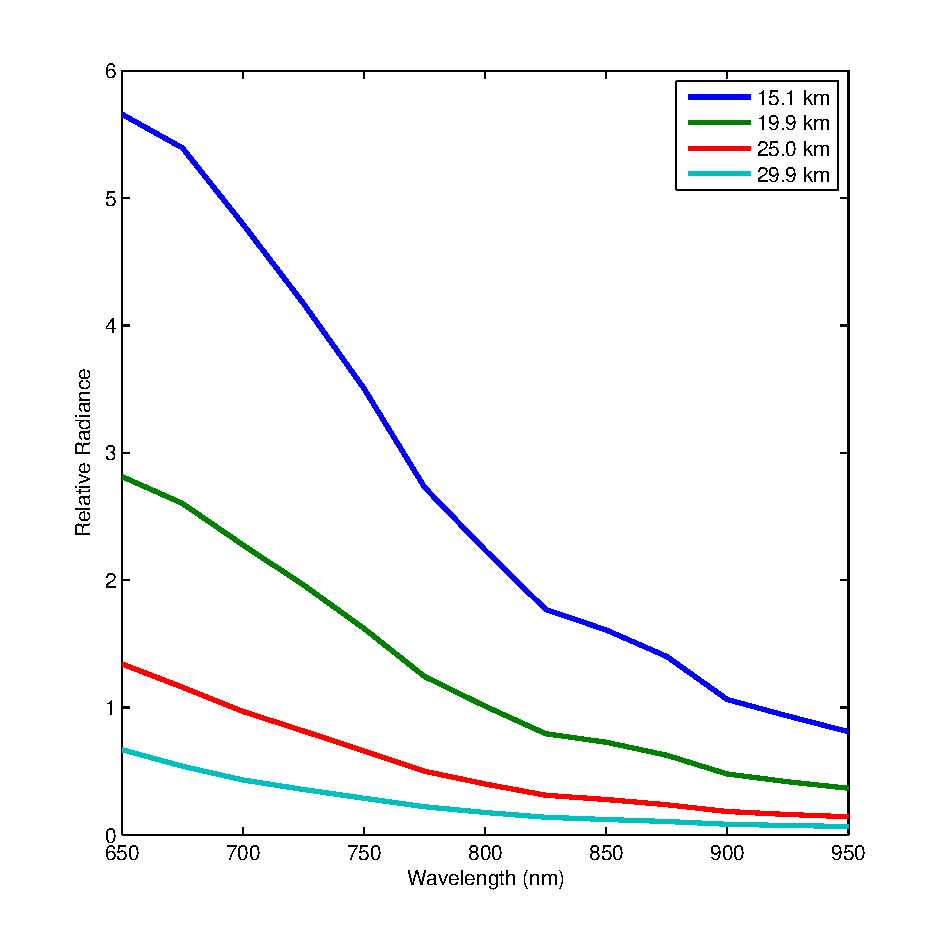
\includegraphics[width=1.0\textwidth]{./Images/5-2-AliSpectralRadiances.pdf}
    \caption[TODO:Write This]{Level 1 relative radiances spectrally from 650~nm to 950~nm as measured form ALI at approximately 14:20 UTC consisting of images number 204 to 216 looking 90\si{\degree} from the sun facing southwards. These spectral profiles are presented at several tangent altitudes with a horizontal field of view of 0\si{\degree}.}
    \label{fig:5.2:AliSpectralRadiances}
\end{figure} 